\section{Method}
\label{sec:method}
% \begin{figure}
%     \centering
%     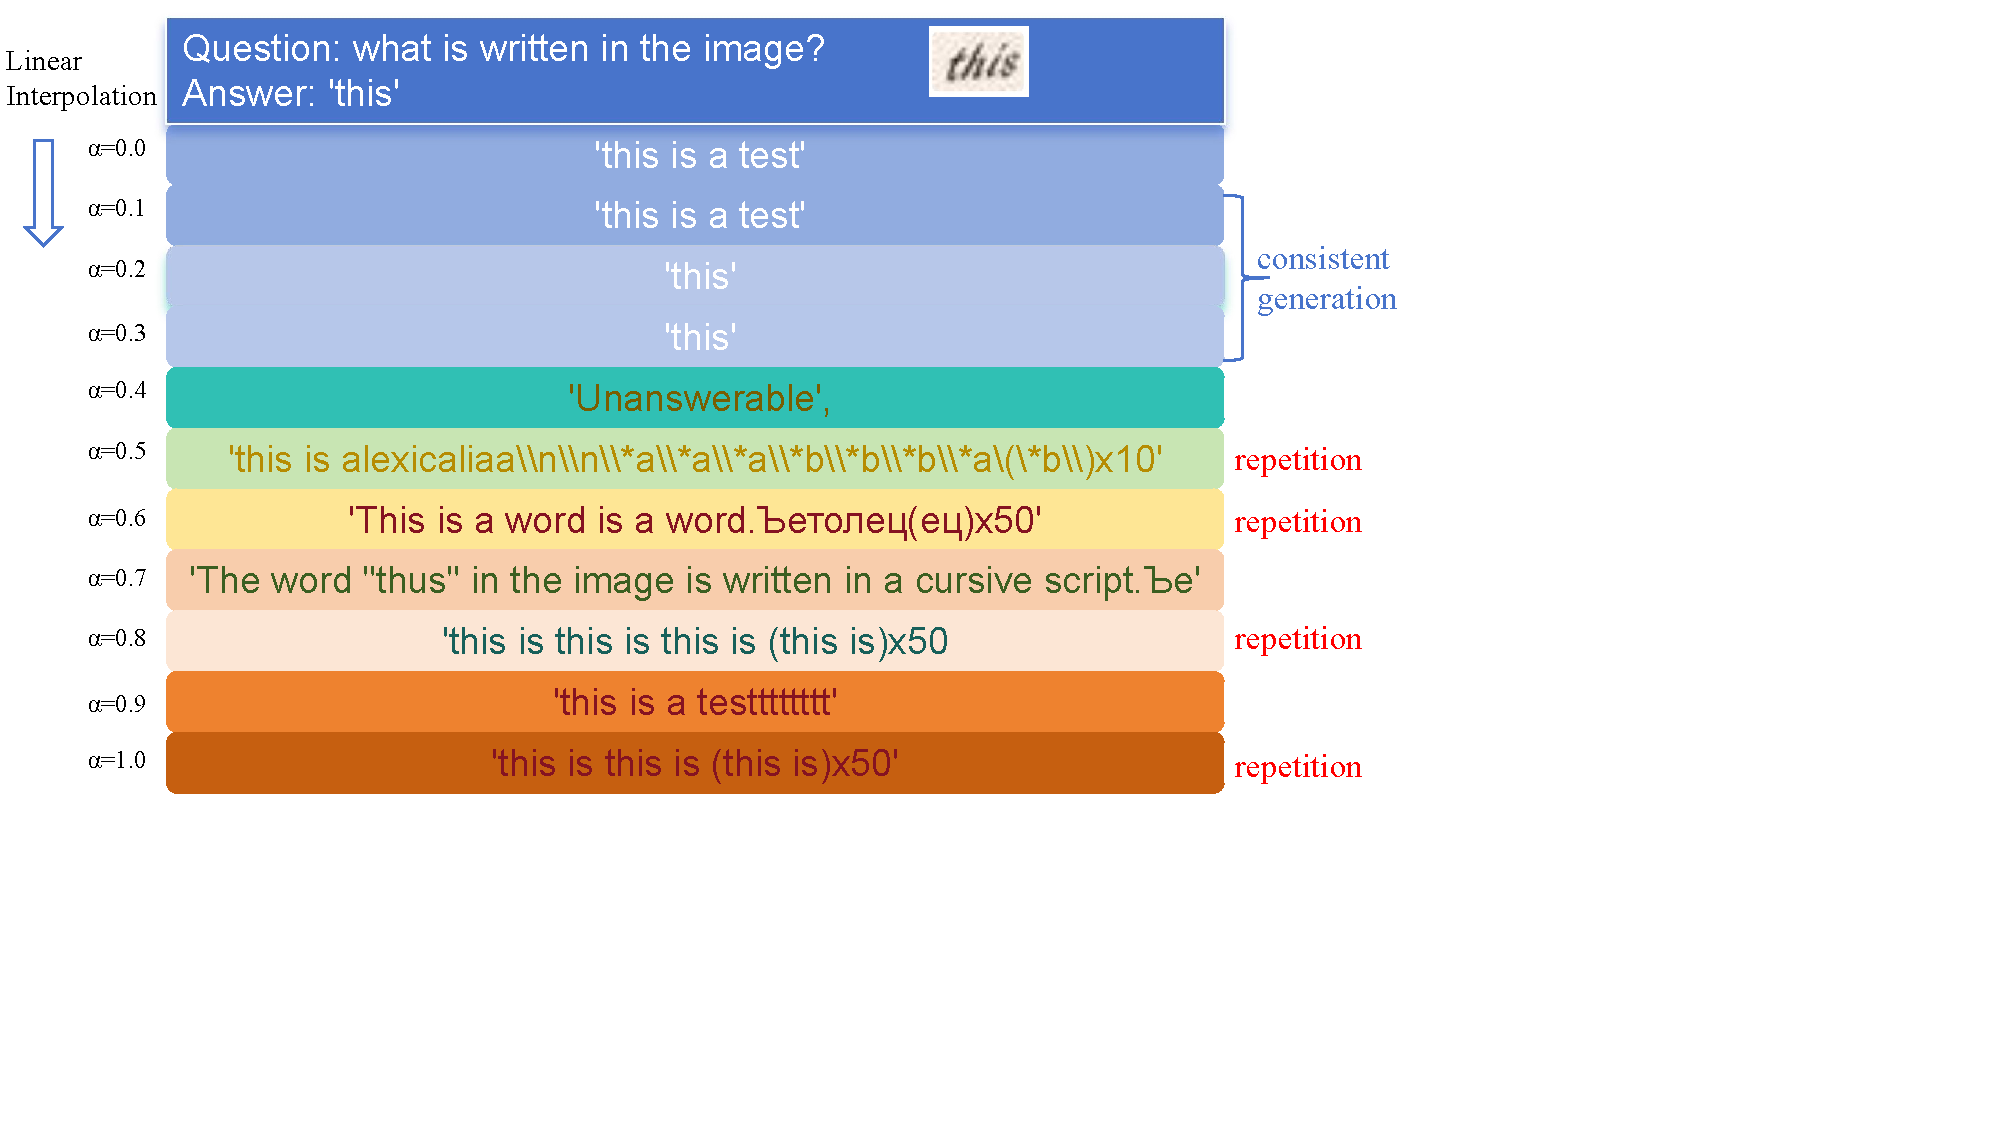
\includegraphics[width=\linewidth]{figure/crop_diff-case.pdf}
%     \caption{Model responses with change of $\alpha$ when doing linear interpolation. Color represents the similarity of responses.  }
%     \label{fig:asymmetry}
% \end{figure}
%这个前提也跟landscpe有关。不是同一个LLM预训练的话,landscape距离太远
%TODO: 这段得改
% The prerequisite for merging homogeneous models is that the models to be merged must have been fine-tuned from the same model. The prerequisite for merging heterogeneous multi-modal models is extended to models that have been continue pretrained from the same LLM. Only under these preconditions will the two models be similar in the landscape, and the fusion operation will yield benefits. Given this premise, our Mms-Merging method follows next three steps to perform merging in any heterogeneous MLLMs.
To tackle the heterogeneous challenges in merging MLLMs, we propose a novel model merging method named \ours. As shown in Figure~\ref{fig:figure1}(a), it involves three steps: mapping, merging and searching. In the mapping step, we define a mapping function that enables the merging of parameters from different architectures. Next, in the merging step, we apply linear interpolation to adaptively optimize the performance on specific downstream tasks. Finally, in the searching step, we design a unsupervised hyper-parameter selection method for choosing linear interpolation coefficient during merging. This method is based on our novel discovery that the model performance in the parameter space can be approximated by the difference among model responses without the need of labeled data.
\subsection{Mapping} \label{mapping}

% To merge the parameters of two heterogeneous models, \( M_1 \) and \( M_2 \), they must first be unified under the same basic architecture. For optimal results, we select the model with superior performance as the basic architecture. Subsequently, a set of mapping rules is defined to retain parameters with similar functions, while discarding dissimilar ones. Mapping rules is defined as follows:
% \begin{equation*}
%     \mathsf{Mapping}(\theta_1, \theta_2) =\left\{
%     \begin{aligned}
%         &\mathsf{True}, \quad & \mathsf{if}  \theta_1 \simeq \theta_2 
%         \\
%         &\mathsf{False}, \quad & \mathsf{else}
%     \end{aligned} \right.
% \end{equation*}
% 尝试了一下别的格式 可以可以好看很多

To merge the parameters of two heterogeneous models $M_1$ and $M_2$ into $M_1$'s architecture, we need to align their parameters by defining a mapping $f$ that maps each parameter $\theta_1$ in $M_1$ to its corresponding parameter $\theta_2$ in $M_2$ (or $\phi$ if there is no such corresponding parameter).
As previously discussed in Section~\ref{mllms}, we only tackle the heterogeneous MLLMs that are designed from same pre-trained language model architecture, but adapts different modifications on model structure.

The principle of designing the mapping $f$ is that for the shared weights between the models (e.g. the weights in the pre-trained model), we can map them directly, and for additional weights in $M_1$, we map it to its original corresponding weight in $M_2$ if it is a duplicated multimodal parameter in $M_1$'s specific design, otherwise we map $\phi$ with it and apply no operation later in merging. In this way, we leverage the additional weights as much as possible without mapping irrelevant parameters together.

% Formally, given two MLLMs that their structure are developed based on the same LLM structure, suppose $M_1$ and $M_2$ has duplicate part of their parameters $\Theta_1$ and $\Theta_2$ for multimodal purpose, which brings additional parameters $\Delta_1 = \{ \theta_1^{a_1}, \ldots, \theta_1^{a_j}\}$ and $\Delta_2 = \{ \theta_2^{b_1}, \ldots, \theta_2^{b_k}\}$ respectively, we define the mapping $f$ as follows:
% \begin{equation}
%     \mathsf{f}(\theta_1^i) =\left\{
%     \begin{aligned}
%         &\theta_2^i,   & \mathsf{if}  \theta_1^i \notin \Delta_1 \And \theta_2^i \in \Theta_2
%         \\
%         &\phi,   & \mathsf{if}  \theta_1^i \notin \Delta_1 \And \theta_2^i \notin \Theta_2
%         \\
%         &\theta_2^{a_j},   & \mathsf{if} \theta_1^i=\theta_1^{a_j} \in \Delta_1 \And \theta_2^{a_j} \in \Delta_2
%         \\
%         &\theta_2^{\mathsf{org}(a_j)},   & \mathsf{if} \theta_1^i=\theta_1^{a_j} \in \Delta_1 \And \theta_2^{a_j} \notin \Delta_2
%         % \\
%         % &\phi,  \quad & \mathsf{otherwise}
%     \end{aligned} \right. \label{eq:mapping}
% \end{equation}
% \noindent where $\mathsf{org}(a_j)$ is the index of the original parameter of the duplicated parameter $\theta_1^{a_j}$ in $M_1$.



\subsection{Merging}
We follow the paradigm in Task Arithmetic \cite{task-arithmetic} to apply merging operation on task vectors and apply linear interpolation on them. 
Task vectors are defined as the fine-tuned parameters subtracted by pre-train weights: $\tau_i = \theta_i - \theta_0 \ (i=1,2)$, where $\theta_1$ and $\theta_2$ is the models to be merged, and $\theta_0$ is their common initialization point (e.g. the shared pre-trained weights for two different finetuned model).
Linear interpolation offers the availability to directly control the tendency between the two models alongside its simplicity. This allows us to actively adapt to different downstream tasks, as different downstream tasks often requires different combination or tendency on the two models for the best performance.
Linear interpolation on task vectors can be simply formatted as:  $\theta_{out} = \theta_0 + (1-\alpha) \tau_1 + \alpha \tau_2$, 
% \begin{align*}
%     &\tau_i = \theta_i - \theta_0 \quad \quad \quad (i=1,2)
%     \\
%     &\theta_{out} = \theta_0 + \alpha \tau_1 + (1-\alpha) \tau_2
% \end{align*}
% \noindent, where $\theta_1$ and $\theta_2$ is the models to be merged, and $\theta_0$ is their common initialization point (e.g. the shared pre-trained weights for two different finetuned model).
\noindent, where $\alpha$ is the linear interpolation coefficient. This is equivalent to: $\theta_{out} = (1-\alpha) \theta_1 + \alpha \theta_2$.
% \[ \theta_{out} = \alpha \theta_1 + (1-\alpha) \theta_2 \]
Thus, leveraging our mapping funciton $f$ in Section~\ref{mapping}, we can apply our merging operation on heterogeneous MLLMs as follow:
\begin{equation}
    \theta_{out}^i =\left\{
    \begin{aligned}
        &\theta_1^i, \quad & \mathsf{if}  f(\theta_1^i) = \phi
        \\
        &(1-\alpha) \theta_1^i + \alpha f(\theta_1^i),  \quad &          \mathsf{otherwise}
        % \\
        % &\phi,  \quad & \mathsf{otherwise}
    \end{aligned} \right.
\end{equation}
Note that $f(\theta_1)$ is the parameter in $M_2$ that corresponds to $\theta_1$, according to the mapping function $f$. Now we can define the merging process of two model parameters $\Theta_1=\{\theta_1^i\}$ and $\Theta_2=\{\theta_2^j\}$ accordingly:
\begin{equation}
    \operatorname*{Merge}(\Theta_1, \Theta_2; f; \alpha) = \{\theta_{out}^i\} \label{eq:merge}
\end{equation}



% 下边是原来的

% We obtained the homogeneous parameter pairs from mapping step. Then by subtracting them from the original LLM weights $\theta_0$, we can obtain the task vector. 
% \[   \tau_i = \theta_i - \theta_0 \quad (i=1,2)\]

% % Note that this modality vector is quite similar to the task vector \cite{task-arithmetic} in homogeneous fusion. However, the task vector is task-related, whereas the modality vector is modality-related.



% The formula for merging \( M_2 \) into \( M_1 \) when doing linear interpolation is as follows:
% % \[
% % \theta = 
% % \begin{cases} 
% % \theta_1, & \hspace{-5em} \text{if }  Mapping(\theta_1, \theta_2) = False \\ 
% % \theta_0 + \alpha \tau_1 + (1-\alpha) \tau_2, &          \hspace{5em}  else 
% % \end{cases}
% % \]

% \begin{equation*}
%     \theta =\left\{
%     \begin{aligned}
%         &\theta_1, \quad & \mathsf{if}  f(\theta_1) = \phi
%         \\
%         &\theta_0 + \alpha \tau_1 + (1-\alpha) \tau_2,  \quad &          \mathsf{otherwise}
%         % \\
%         % &\phi,  \quad & \mathsf{otherwise}
%     \end{aligned} \right.
% \end{equation*}
% , where \( \theta_0 \in M_0, \theta_1 \in M_1, \theta_2 \in M_2 \), \(\alpha\) is a scaling hyperparameter (as used in past work \cite{task-arithmetic}).. Both \( M_1\) and \( M_2\) are continuously pre-trained from the same LLM, \( M_0\).  This equation represents the interpolated value \( W \) based on the blend of \( \theta_1 \) and \( \theta_2 \) controlled by the parameter \( \alpha \), merging into \( \theta_2 \) unless the condition defined by the function \text{mapping} is true.





\subsection{Searching} \label{searching}

% actively 需要搜索

Consider the base model, which is defined as the architecture that will be used after the merging process, containing $N$ scalar weight elements, then the merging process can be seen as the operation on a $N$-dimentional vector space $\mathbb{R}^N$, where the merging strategy $F$ transform two input points as initial parameters $\Theta_1$ and $\Theta_2$ to the merged parameters $\Theta_{out}$. For simplicity, we consider the case when the merging strategy $F$ takes one hyper-parameter $\alpha$ (linear interpolation coefficient).
\[
\Theta_{out} = F(\Theta_1, \Theta_2; \alpha), \quad \Theta_1, \Theta_2, \Theta_{out} \in \mathbb{R}^N
\]
Given the inputs $t_i$ on a downstream task, this creates a landscape on $\mathbb{R}^N$ that each model parameter corresponds to the model performance $S_{t_i}$ on the inputs.
\[
S_{t_i}(\Theta_{out}) = S_{t_i, F}(\Theta_1, \Theta_2, \alpha)
\]
Therefore, the goal of the hyper-parameter searching is to find the best $\alpha$ that maximize the merged model's performance on the tasks. For simplicity, we omit the F in the index.
\[
\alpha^* = \operatorname*{argmax}_{\alpha}(S_{t_i}(\Theta_1, \Theta_2, \alpha))
\]
Note that as the landscape varies greatly in different tasks, the best $\alpha$ may be different as well.


% \noindent\textbf{Performance Estimation} \  
Previous model merging methods mainly relies on a validation set to search for the best hyper-parameter $\alpha$ with supervised searching. Formally, they use the best $\alpha$ in validation set $\hat{t_i}$ to approximate the best $\alpha$ in test set $t_i$.
\[
\hat{\alpha} = \operatorname*{argmax}_{\alpha}(S_{\mathbf{\hat{t_i}}}(\Theta_1, \Theta_2, \alpha)) \approx \operatorname*{argmax}_{\alpha}(S_{\mathbf{t_i}}(\Theta_1, \Theta_2, \alpha))
\]

However, this supervised way of searching has certain disadvantages: (1) labeled data with ground truth is hard to collect in some scenarios, and (2) the distribution shift between the validation set and the test set, even on the same task, will interfere the selection of the best hyper-parameter $\alpha^*$. To get rid of these drawbacks, we propose an unsupervised hyper-parameter selection method through a performance estimation metric that requires no labeled data.

Specifically, we discover that the difference of generated responses between two adjacent $\alpha$ candidates can be used to estimate the model performance, and the best $\alpha$ can be approximated by the one with the lowest adjacent difference. 
As shown in Figure~\ref{fig:difference}, the trend of model performance is similar with its generation consistency which is measured by response differences, and the $\alpha$ with the highest generation consistency match the $\alpha$ with the highest performance.
Formally, let $\alpha^-$ and $\alpha^+$ be adjacent candidates on both sides of $\alpha$, respectively, and $D_{t_i}(\alpha; \alpha^-, \alpha^+)$ denoting the difference of generated responses between , we take:
\[
\bar{\alpha} = \operatorname*{argmin}_{\alpha}(D_{t_i}(\alpha; \alpha^-, \alpha^+)) \approx \operatorname*{argmax}_{\alpha}(S_{t_i}(\Theta_1, \Theta_2, \alpha))
\]
as the approximation of the best choice for $\alpha$. This eliminates the need of labeled data with ground truth, and avoids the data distribution shift between validation set and test set. 

The discovery indicates that near the best performance point, the model response tends to be more stable. This can be explained via a convex hypothesis. Suppose the landscape on given task $t_i$ is convex in a subspace of the parameter space that covers the candidate results of merged models, that is, for any $\lambda \in [0,1]$ we have:
\begin{equation*}
    S_{t_i}(\lambda\Theta_1+(1-\lambda)\Theta_2) \geq \
     S_{t_i}(\lambda\Theta_1) + \
      S_{t_i}((1-\lambda)\Theta_2)
\end{equation*}
This guarantee that the optimum is attained where the gradient vanishes:
\begin{equation*}
    \nabla_{\Theta}S_{t_i}(\Theta^*) = 0
\end{equation*}
where $\Theta^* \in \mathbb{R}^N$ is the optimal parameter value. In a convex function, the Hessian $H(\Theta^*)=\nabla^2_{\Theta}S_{t_i}(\Theta^*)$ at the optimum $\Theta^*$ is positive semi-definite, which implies local stability in a neighborhood around $\Theta^*$. The stability can be characterized by the second-order Taylor expansion:
\begin{equation*}
    S_{t_i}(\Theta) \approx S_{t_i}(\Theta^*) + \frac{1}{2}(\Theta-\Theta^*)^{\top}H(\Theta^*)(\Theta-\Theta^*)
\end{equation*}
Since $H(\Theta^*) \geq 0$, small deviations from $\Theta^*$ will result in small increases in the performance, ensuring relative stability on the landscape. Although the convex hypothesis is ideal, we confirm the effectiveness of our unsupervised hyper-parameter selection method in various experiments.
Proof in Appendix~\ref{appendix:proof} further shows the relationship between generation consistency and model performance.

%尽管真实情况可能有出入,但可以看做微小扰动不影响结果(或者有多个local minimum),或者和D不一致,并且我们在后续实验中证明了这种估计是有效果的


We also find that while the landscape often changes between the validation and test sets and across different tasks, it remains consistent between the full test set and a small subset. This suggests that we can perform unsupervised hyper-parameter selection on a smaller subset of the data $\bar{t_i}$ without compromising its accuracy.
%TODO:两个landscape相似的公式
\[
\bar{\alpha} = \operatorname*{argmin}_{\alpha}(D_{\mathbf{\bar{t_i}}}(\alpha; \alpha^-, \alpha^+)) \approx \operatorname*{argmax}_{\alpha}(S_{\mathbf{t_i}}(\theta_1, \theta_2, \alpha))
\]

In conclusion, the process of \ours is described in Algorithm~\ref{alg:composition}.

% notation of 'gradient' G as vector

% 目标是说明越稳定的地方越好

% 但是这个 gradient 不可知。但我们在实验中discover到difference是一个好的指标

% 用于估计 D ~ G

% 给出 algorithm

% 误差分析

% 尽管在真实情况中这个假设会有扰动,但实验表明我们的方法是优秀的。并不一定能选到最好的,但是可以在最好的附近。

\begin{algorithm}
\caption{\ours Procedure}
\label{alg:composition}
\begin{algorithmic}[1]
\Require Original MLLMs $M_1, M_2$, their parameters $\Theta_1, \Theta_2$ respectively, a subset of test inputs $\bar{t}$, and the candidates of the hyper-parameter $\{\alpha_n\}$
\Ensure Merged parameters $\Theta_{\text{out}}$ on $M_1$'s architecture

% \State Initialize $\Theta_{\text{common}}$ and $\Theta_{\text{compose}}$ as empty sets
% TODO: add indicator of the three stages
 \State Define a mapping $f$ that maps each parameter $\theta_1$ in $M_1$ architecture with its corresponding parameter $\theta_2$ in $M_2$ architecture (if exists) \Comment{Section~\ref{mapping}}
\State Define a process $\operatorname*{Generate}(\Theta, \bar{t})$ that returns the generation responses $G$ of model with parameters $\Theta$ on inputs $\bar{t}$
\State Define a function $\operatorname*{DiffCnt}(G_i, G_j)$ that counts the number of corresponding elements in $G_i$ and $G_j$ that do not exactly match
% TODO: \State 
\For{$i = 1$ to $n$}
    \For{each hyper-parameter candidate $\alpha_i$ in $\{\alpha_n\}$}
        \State $\Theta_{cand}^{i} \gets \operatorname*{Merge}(\Theta_1, \Theta_2; f; \alpha_i)$ \Comment{Equation \eqref{eq:merge}}
        \State $G_i \gets \operatorname*{Generate}(\Theta_{cand}^{i}, \bar{t})$
    \EndFor
\EndFor
\For{$i = 2$ to $n-1$} \Comment{Assuming $\{\alpha_n\}$ is monotonic}
    \For{each hyper-parameter candidate $\alpha_i$ in $\{\alpha_n\}$}
        \State $D_i \gets \operatorname*{DiffCnt}(G_i, G_{i-1}) + \operatorname*{DiffCnt}(G_i, G_{i+1})$
        % \Comment{sf}
    \EndFor
\EndFor
\State $i^* \gets \operatorname*{argmin}_{i}(D_i)$
\State $\Theta_{\text{out}} \gets \Theta_{\text{cand}}^{i^*}$
\State \Return $\Theta_{\text{out}}$
\end{algorithmic}
\end{algorithm}

% TODO: 修改 algorithm 里边两个未定义,并且之前公式里的一大堆问题,见鹏导的pdf